% Created by tikzDevice version 0.12.6 on 2024-04-16 16:15:50
% !TEX encoding = UTF-8 Unicode
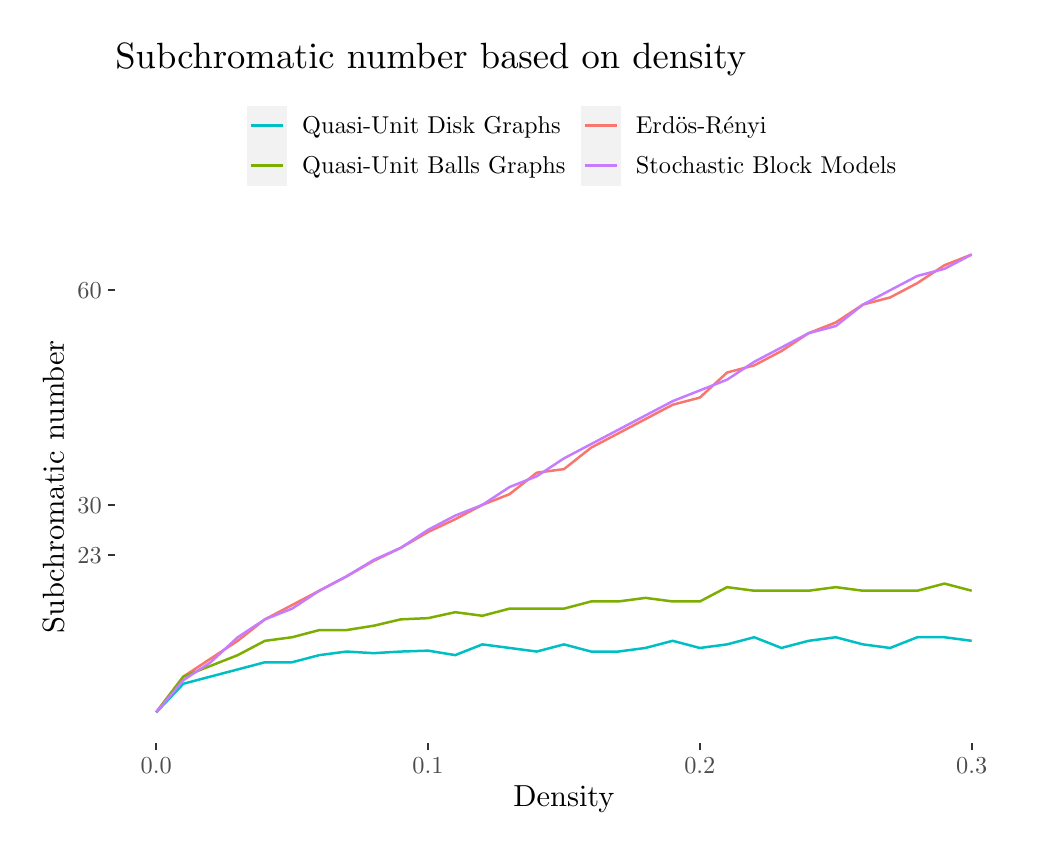
\begin{tikzpicture}[x=1pt,y=1pt]
\definecolor{fillColor}{RGB}{255,255,255}
\path[use as bounding box,fill=fillColor,fill opacity=0.00] (0,0) rectangle (361.35,289.08);
\begin{scope}
\path[clip] (  0.00,  0.00) rectangle (361.35,289.08);
\definecolor{drawColor}{RGB}{255,255,255}
\definecolor{fillColor}{RGB}{255,255,255}

\path[draw=drawColor,line width= 0.6pt,line join=round,line cap=round,fill=fillColor] (  0.00,  0.00) rectangle (361.35,289.08);
\end{scope}
\begin{scope}
\path[clip] ( 31.71, 30.69) rectangle (355.85,215.51);
\definecolor{fillColor}{RGB}{255,255,255}

\path[fill=fillColor] ( 31.71, 30.69) rectangle (355.85,215.51);
\definecolor{drawColor}{RGB}{248,118,109}

\path[draw=drawColor,line width= 0.9pt,line join=round] ( 46.45, 41.67) --
	( 56.27, 54.60) --
	( 66.09, 61.06) --
	( 75.91, 67.52) --
	( 85.74, 75.28) --
	( 95.56, 80.45) --
	(105.38, 85.62) --
	(115.20, 90.79) --
	(125.02, 96.41) --
	(134.85,101.13) --
	(144.67,106.83) --
	(154.49,111.47) --
	(164.31,116.64) --
	(174.14,120.52) --
	(183.96,128.27) --
	(193.78,129.56) --
	(203.60,137.32) --
	(213.43,142.49) --
	(223.25,147.66) --
	(233.07,152.83) --
	(242.89,155.41) --
	(252.72,164.46) --
	(262.54,167.05) --
	(272.36,172.22) --
	(282.18,178.68) --
	(292.00,182.56) --
	(301.83,189.02) --
	(311.65,191.60) --
	(321.47,196.77) --
	(331.29,203.24) --
	(341.12,207.11);
\definecolor{drawColor}{RGB}{124,174,0}

\path[draw=drawColor,line width= 0.9pt,line join=round] ( 46.45, 41.67) --
	( 56.27, 54.60) --
	( 66.09, 58.47) --
	( 75.91, 62.35) --
	( 85.74, 67.52) --
	( 95.56, 68.81) --
	(105.38, 71.40) --
	(115.20, 71.40) --
	(125.02, 72.97) --
	(134.85, 75.28) --
	(144.67, 75.71) --
	(154.49, 77.86) --
	(164.31, 76.57) --
	(174.14, 79.15) --
	(183.96, 79.15) --
	(193.78, 79.15) --
	(203.60, 81.74) --
	(213.43, 81.74) --
	(223.25, 83.03) --
	(233.07, 81.74) --
	(242.89, 81.74) --
	(252.72, 86.91) --
	(262.54, 85.62) --
	(272.36, 85.62) --
	(282.18, 85.62) --
	(292.00, 86.91) --
	(301.83, 85.62) --
	(311.65, 85.62) --
	(321.47, 85.62) --
	(331.29, 88.20) --
	(341.12, 85.62);
\definecolor{drawColor}{RGB}{0,191,196}

\path[draw=drawColor,line width= 0.9pt,line join=round] ( 46.45, 41.67) --
	( 56.27, 52.01) --
	( 66.09, 54.60) --
	( 75.91, 57.18) --
	( 85.74, 59.77) --
	( 95.56, 59.77) --
	(105.38, 62.35) --
	(115.20, 63.64) --
	(125.02, 63.06) --
	(134.85, 63.64) --
	(144.67, 63.97) --
	(154.49, 62.35) --
	(164.31, 66.23) --
	(174.14, 64.94) --
	(183.96, 63.64) --
	(193.78, 66.23) --
	(203.60, 63.64) --
	(213.43, 63.64) --
	(223.25, 64.94) --
	(233.07, 67.52) --
	(242.89, 64.94) --
	(252.72, 66.23) --
	(262.54, 68.81) --
	(272.36, 64.94) --
	(282.18, 67.52) --
	(292.00, 68.81) --
	(301.83, 66.23) --
	(311.65, 64.94) --
	(321.47, 68.81) --
	(331.29, 68.81) --
	(341.12, 67.52);
\definecolor{drawColor}{RGB}{199,124,255}

\path[draw=drawColor,line width= 0.9pt,line join=round] ( 46.45, 41.67) --
	( 56.27, 53.30) --
	( 66.09, 59.77) --
	( 75.91, 68.81) --
	( 85.74, 75.28) --
	( 95.56, 79.15) --
	(105.38, 85.62) --
	(115.20, 90.79) --
	(125.02, 96.74) --
	(134.85,101.13) --
	(144.67,107.62) --
	(154.49,112.76) --
	(164.31,116.64) --
	(174.14,123.10) --
	(183.96,126.98) --
	(193.78,133.44) --
	(203.60,138.61) --
	(213.43,143.78) --
	(223.25,148.95) --
	(233.07,154.12) --
	(242.89,158.00) --
	(252.72,161.88) --
	(262.54,168.34) --
	(272.36,173.51) --
	(282.18,178.68) --
	(292.00,181.26) --
	(301.83,189.02) --
	(311.65,194.19) --
	(321.47,199.36) --
	(331.29,201.94) --
	(341.12,207.11);
\end{scope}
\begin{scope}
\path[clip] (  0.00,  0.00) rectangle (361.35,289.08);
\definecolor{drawColor}{gray}{0.30}

\node[text=drawColor,anchor=base east,inner sep=0pt, outer sep=0pt, scale=  0.88] at ( 26.76, 95.51) {23};

\node[text=drawColor,anchor=base east,inner sep=0pt, outer sep=0pt, scale=  0.88] at ( 26.76,113.61) {30};

\node[text=drawColor,anchor=base east,inner sep=0pt, outer sep=0pt, scale=  0.88] at ( 26.76,191.16) {60};
\end{scope}
\begin{scope}
\path[clip] (  0.00,  0.00) rectangle (361.35,289.08);
\definecolor{drawColor}{gray}{0.20}

\path[draw=drawColor,line width= 0.6pt,line join=round] ( 28.96, 98.54) --
	( 31.71, 98.54);

\path[draw=drawColor,line width= 0.6pt,line join=round] ( 28.96,116.64) --
	( 31.71,116.64);

\path[draw=drawColor,line width= 0.6pt,line join=round] ( 28.96,194.19) --
	( 31.71,194.19);
\end{scope}
\begin{scope}
\path[clip] (  0.00,  0.00) rectangle (361.35,289.08);
\definecolor{drawColor}{gray}{0.20}

\path[draw=drawColor,line width= 0.6pt,line join=round] ( 46.45, 27.94) --
	( 46.45, 30.69);

\path[draw=drawColor,line width= 0.6pt,line join=round] (144.67, 27.94) --
	(144.67, 30.69);

\path[draw=drawColor,line width= 0.6pt,line join=round] (242.89, 27.94) --
	(242.89, 30.69);

\path[draw=drawColor,line width= 0.6pt,line join=round] (341.12, 27.94) --
	(341.12, 30.69);
\end{scope}
\begin{scope}
\path[clip] (  0.00,  0.00) rectangle (361.35,289.08);
\definecolor{drawColor}{gray}{0.30}

\node[text=drawColor,anchor=base,inner sep=0pt, outer sep=0pt, scale=  0.88] at ( 46.45, 19.68) {0.0};

\node[text=drawColor,anchor=base,inner sep=0pt, outer sep=0pt, scale=  0.88] at (144.67, 19.68) {0.1};

\node[text=drawColor,anchor=base,inner sep=0pt, outer sep=0pt, scale=  0.88] at (242.89, 19.68) {0.2};

\node[text=drawColor,anchor=base,inner sep=0pt, outer sep=0pt, scale=  0.88] at (341.12, 19.68) {0.3};
\end{scope}
\begin{scope}
\path[clip] (  0.00,  0.00) rectangle (361.35,289.08);
\definecolor{drawColor}{RGB}{0,0,0}

\node[text=drawColor,anchor=base,inner sep=0pt, outer sep=0pt, scale=  1.10] at (193.78,  7.64) {Density};
\end{scope}
\begin{scope}
\path[clip] (  0.00,  0.00) rectangle (361.35,289.08);
\definecolor{drawColor}{RGB}{0,0,0}

\node[text=drawColor,rotate= 90.00,anchor=base,inner sep=0pt, outer sep=0pt, scale=  1.10] at ( 13.08,123.10) {Subchromatic number};
\end{scope}
\begin{scope}
\path[clip] (  0.00,  0.00) rectangle (361.35,289.08);
\definecolor{fillColor}{RGB}{255,255,255}

\path[fill=fillColor] ( 68.21,226.51) rectangle (319.36,266.42);
\end{scope}
\begin{scope}
\path[clip] (  0.00,  0.00) rectangle (361.35,289.08);
\definecolor{fillColor}{gray}{0.95}

\path[fill=fillColor] ( 79.21,246.47) rectangle ( 93.66,260.92);
\end{scope}
\begin{scope}
\path[clip] (  0.00,  0.00) rectangle (361.35,289.08);
\definecolor{drawColor}{RGB}{0,191,196}

\path[draw=drawColor,line width= 0.9pt,line join=round] ( 80.65,253.70) -- ( 92.22,253.70);
\end{scope}
\begin{scope}
\path[clip] (  0.00,  0.00) rectangle (361.35,289.08);
\definecolor{fillColor}{gray}{0.95}

\path[fill=fillColor] ( 79.21,232.01) rectangle ( 93.66,246.47);
\end{scope}
\begin{scope}
\path[clip] (  0.00,  0.00) rectangle (361.35,289.08);
\definecolor{drawColor}{RGB}{124,174,0}

\path[draw=drawColor,line width= 0.9pt,line join=round] ( 80.65,239.24) -- ( 92.22,239.24);
\end{scope}
\begin{scope}
\path[clip] (  0.00,  0.00) rectangle (361.35,289.08);
\definecolor{fillColor}{gray}{0.95}

\path[fill=fillColor] (199.84,246.47) rectangle (214.29,260.92);
\end{scope}
\begin{scope}
\path[clip] (  0.00,  0.00) rectangle (361.35,289.08);
\definecolor{drawColor}{RGB}{248,118,109}

\path[draw=drawColor,line width= 0.9pt,line join=round] (201.28,253.70) -- (212.85,253.70);
\end{scope}
\begin{scope}
\path[clip] (  0.00,  0.00) rectangle (361.35,289.08);
\definecolor{fillColor}{gray}{0.95}

\path[fill=fillColor] (199.84,232.01) rectangle (214.29,246.47);
\end{scope}
\begin{scope}
\path[clip] (  0.00,  0.00) rectangle (361.35,289.08);
\definecolor{drawColor}{RGB}{199,124,255}

\path[draw=drawColor,line width= 0.9pt,line join=round] (201.28,239.24) -- (212.85,239.24);
\end{scope}
\begin{scope}
\path[clip] (  0.00,  0.00) rectangle (361.35,289.08);
\definecolor{drawColor}{RGB}{0,0,0}

\node[text=drawColor,anchor=base west,inner sep=0pt, outer sep=0pt, scale=  0.88] at ( 99.16,250.67) {Quasi-Unit Disk Graphs};
\end{scope}
\begin{scope}
\path[clip] (  0.00,  0.00) rectangle (361.35,289.08);
\definecolor{drawColor}{RGB}{0,0,0}

\node[text=drawColor,anchor=base west,inner sep=0pt, outer sep=0pt, scale=  0.88] at ( 99.16,236.21) {Quasi-Unit Balls Graphs};
\end{scope}
\begin{scope}
\path[clip] (  0.00,  0.00) rectangle (361.35,289.08);
\definecolor{drawColor}{RGB}{0,0,0}

\node[text=drawColor,anchor=base west,inner sep=0pt, outer sep=0pt, scale=  0.88] at (219.79,250.67) {Erdös-Rényi};
\end{scope}
\begin{scope}
\path[clip] (  0.00,  0.00) rectangle (361.35,289.08);
\definecolor{drawColor}{RGB}{0,0,0}

\node[text=drawColor,anchor=base west,inner sep=0pt, outer sep=0pt, scale=  0.88] at (219.79,236.21) {Stochastic Block Models};
\end{scope}
\begin{scope}
\path[clip] (  0.00,  0.00) rectangle (361.35,289.08);
\definecolor{drawColor}{RGB}{0,0,0}

\node[text=drawColor,anchor=base west,inner sep=0pt, outer sep=0pt, scale=  1.32] at ( 31.71,274.49) {Subchromatic number based on density};
\end{scope}
\end{tikzpicture}
